\chapter{Analysis}
In this chapter the analysis method will be described according to the three phases in the methodology chapter. Observations during these phases is used in the analysis phase to more efficient. results in this chapter is only presented as arguments to limit the data needed to be processed and included in the human-learn:Rule-based process. This manual pre-filtering is done based on network knowledge or observations or each device in the smart home environment.

\subsection{Phase 1 analysis}
Pre-filtering in phase one uses the standby traffic captured. All traffic sent from or to the robot vacuum cleaner is the time period, 8 January 20:00 to 22 January 20:00, is included. As a live network has a lot of protocols running to keep the functionality such as, DHCP, ARP, NTP, DNS, SNMP, it is possible to filter out the kind of protocols which is not relevant. 

\paragraph{Address resolution protocol, RFC826}
ARP traffic is used to bind MAC-addresses to higher OSI layer addresses such as IP-addresses. This will only have an effect if there is corresponding devices on the WLAN or LAN as the robot vacuum cleaner. In this thesis there will not be any devices connected to the same network and the ARP requests between the WAN-address and the home router will be on a separate LAN and therefore not relevant.\cite{rfc826}

On all analysis further the filter "not arp" will be applied. This filtered out 24.6 present of all packages in the capture.  

Figure, no APR between BC domains.

\paragraph{Network Time Protocol RFC 958,}
If a network should work the best way as possible, the local time on the communication devices should be in synchronization. NTP is used for this purpose. This is a common protocol and public time servers are used for this purpose. NTP traffic will therefore also be excluded. In standby packet capture it is 0.4 percent NTP packages.\cite{rfc958_ntp}

"not ntp" is applied. 

\paragraph{Dynamic Host Configuration Protocol, RFC 2131}
As for DHCP, both the access-point and the Robot vacuum cleaner as been assigned a reserved IP address in the local DHCP scope. DHCP-traffic will therefore not have any impact or effect on the events. It is therefore not included. "not dhcp" is applied. \cite{rfc2131_dhcp}

Figure DHCP configuration, two gateways

\paragraph{Domain Name System, RFC 1035}
DNS system is a huge part of network communication. All traffic for an IP-address, not hardcoded will have to resolve FQDNs with DNS. This can be a good indication of which FQDNs devices inside the network is trying to communicate with. This will also apply for Irobot.public services. DNS will therefore be included in the analysis. 

Figure Domain Name system

\begin{figure}[!ht]
    \centering
    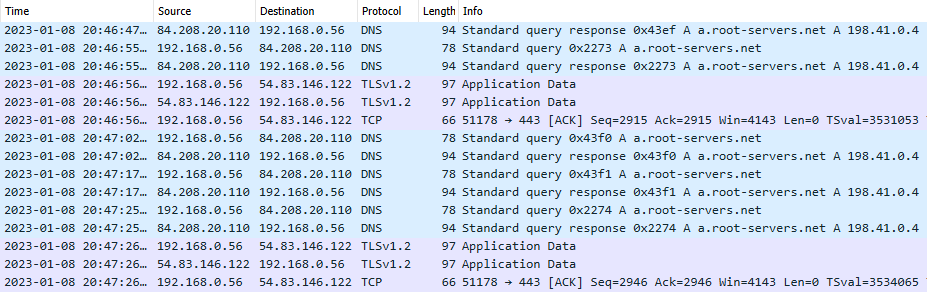
\includegraphics[width=\textwidth]{figures/Wireshark_standby_reoccuring.png}
    \caption{Reoccuring pattern in Standby traffic}
    \label{fig:WSR}
\end{figure}

There is continuous traffic sent towards the configured DNS server requesting A record for a.root-servers.net. According to TP-Link access point this is a mechanism to validate Internet connectivity. If a DNS response with A record it will report as online. This traffic is generated by the TP-Link access point it self and is therefore not relevant for this thesis. 
\begin{itemize}
    \item \textbf{n-devs-gw.tplinkcloud.com}
    \item \textbf{n-deventry-gw.tplinkcloud.com}
\end{itemize}
The IP addresses in the response record can be used in a filter, to remove all traffic not created by the vacuum cleaner. 


If we filter away the DNS traffic there is only application traffic left. As illustrated in figure XX. Since normal smart home devices are behind NAT, the traffic needs to be initiated from the vacuum cleaner it self. Any TCP connections needs to continuously send keep alive packets to keep the communication channel open. Since some of the functionality need s to be initiated from the application via the cloud service. 

\begin{figure}[!ht]
    \centering
    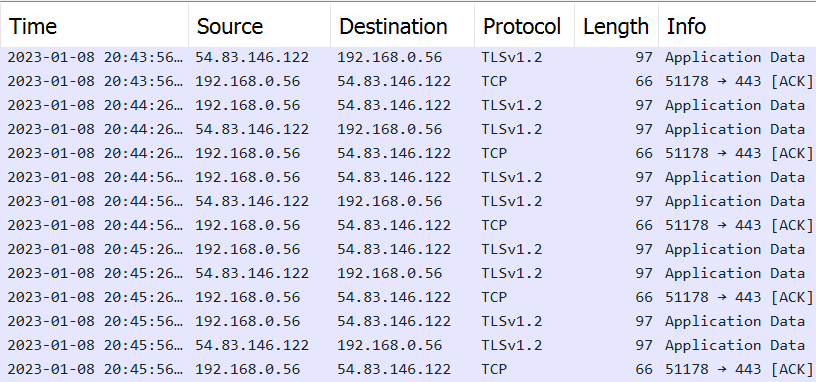
\includegraphics[width=\textwidth]{figures/Wireshark_standby_noDNS.png}
    \caption{Reoccuring pattern application data}
    \label{fig:SBnDNS}
\end{figure}

Figure Keep alive TCP

There is 5 DNS request towards irobot's domain, reoccurring every day. That is: 
\begin{itemize}
    \item \textbf{0.irobot.pool.ntp.org}
    \item \textbf{0.irobot.pool.ntp.org}
    \item \textbf{disc-prod.iot.irobotapi.com}
    \item \textbf{unauth1.prod.iot.irobotapi.com}
    \item \textbf{a2uowfjvhio0fa.iot.us-east-1.amazonaws.com}
\end{itemize}

The continuous TCP keep alive packets are sent to the IP-address in the reply for \textbf{a2uowfjvhio0fa.iot.us-east-1.amazonaws.com}. These IP-addresses and DNS response can be used to identify the correct communication channel used to send commands to the vacuum cleaner. These requests will occure once every day, and the corresponding IP-address will also change, due to DNS load-balancing. 